\begin{figure}[ht]
    \caption{Функции активации на основе Swish}
    \label{act_func_graph}
    \centering
    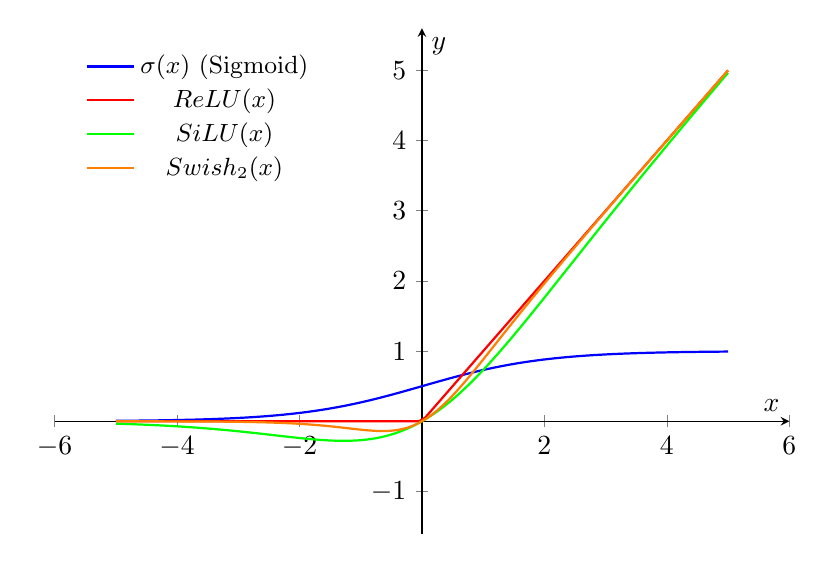
\begin{tikzpicture}
        \begin{axis}[
            width=0.9\textwidth, height=8cm,
            xlabel={$x$},
            ylabel={$y$},
            xmin=-5, xmax=5,
            ymin=-1, ymax=5,
            domain=-5:5,
            samples=100,
            % grid=both,
            legend pos=north west,
            legend style={draw=none, font=\small},
            axis lines=center,
            enlargelimits=true,
            clip=false
        ]
        
        % Sigmoid function
        \addplot[blue, thick] {1 / (1 + exp(-x))};
        \addlegendentry{$\sigma(x)$ (Sigmoid)}
        
        % ReLU function
        \addplot[red, thick] {max(0, x)};
        \addlegendentry{$\text{ReLU}(x)$}
        
        % SiLU function (x * sigmoid(x))
        \addplot[green, thick] {x / (1 + exp(-x))};
        \addlegendentry{$\text{SiLU}(x)$}
        
        % Swish function (x * sigmoid(beta * x), beta = 1)
        \addplot[orange, thick] {x / (1 + exp(-2 * x))};
        \addlegendentry{$\text{Swish}_2(x)$}
        
        
        \end{axis}
    \end{tikzpicture}
    
\end{figure}